\documentclass[tikz, border=10pt]{standalone}
\usepackage{fontspec}

\begin{document}

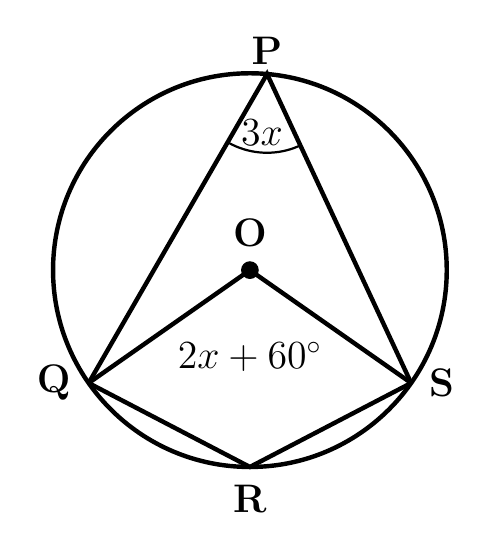
\begin{tikzpicture}[scale=1.0]

% 1. Circle
\draw[ultra thick] (0,0) circle (2.5cm);

% 2. Center point O
\filldraw (0,0) circle (3pt);
\node[above, yshift=5pt, font=\Large\bfseries] at (0,0) {O};

% 3. Coordinates
\coordinate (P) at (85:2.5);
\coordinate (Q) at (215:2.5);
\coordinate (S) at (325:2.5);
\coordinate (R) at (270:2.5);

% 4. Drawing segments
\draw[ultra thick] (Q) -- (P) -- (S);
\draw[ultra thick] (Q) -- (R) -- (S);
\draw[ultra thick] (Q) -- (0,0) -- (S);

% 5. Labels for vertices
\node[above, font=\Large\bfseries] at (P) {P};
\node[left, xshift=-3pt, font=\Large\bfseries] at (Q) {Q};
\node[below, yshift=-3pt, font=\Large\bfseries] at (R) {R};
\node[right, xshift=3pt, font=\Large\bfseries] at (S) {S};

% 6. Refined Angle arc at P (larger arc to accommodate text)
\begin{scope}
    \clip (Q) -- (P) -- (S) -- cycle;
    \draw[thick] (P) circle (1.0cm);
\end{scope}

% 3x moved "UP" and centered within the larger arc
\node[font=\Large\bfseries] at (85:1.75) {$3x$};

% 2x + 60 moved "DOWN" and centered between O and the bottom chords
\node[font=\Large\bfseries, fill=white, inner sep=1.5pt] at (0,-1.1) {$2x + 60^{\circ}$};

\end{tikzpicture}

\end{document}
